\subsection{Interpretabilidad}

The data provided by the platforms have a large volume, because as we mentioned earlier, they are collected
as many data as possible. This document will have multiple samples for which
A set of fields is specified. These sets of fields are similar to each other, but they do not have to be identical.
From these data, a selection of the relevant samples should be made, and of these, the fields necessary to represent
a specific information.


Below we can see several examples the first one is taken from the European open data portal
\footnote{\url{https://tinyurl.com/y3d76525}} and the second of the North American open data portal\footnote{\url{https://data.cityofnewyork.us/api/views/kku6-nxdu/rows.json?accessType=DOWNLOAD}}.

\begin{figure}[h]
    \centering
    \subfigure[EEUU Open Portal.Demographic Statistics By Zip Code]
     {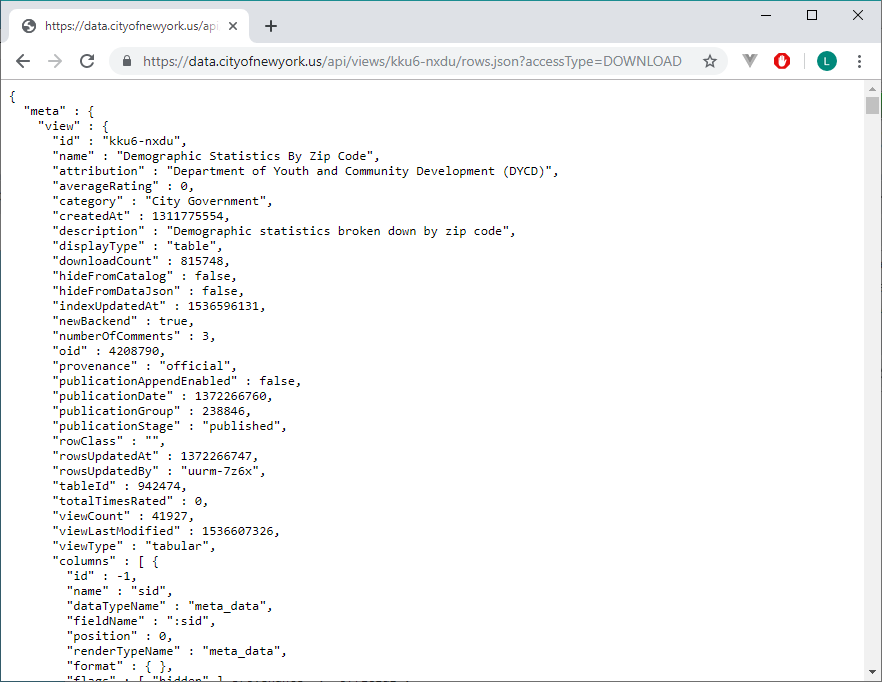
\includegraphics[width=5cm]{ExampleOpenDataEEUU}}
    \hfill
     \subfigure[European Open Data Portal. Air pollutant concentrations 2015]
    {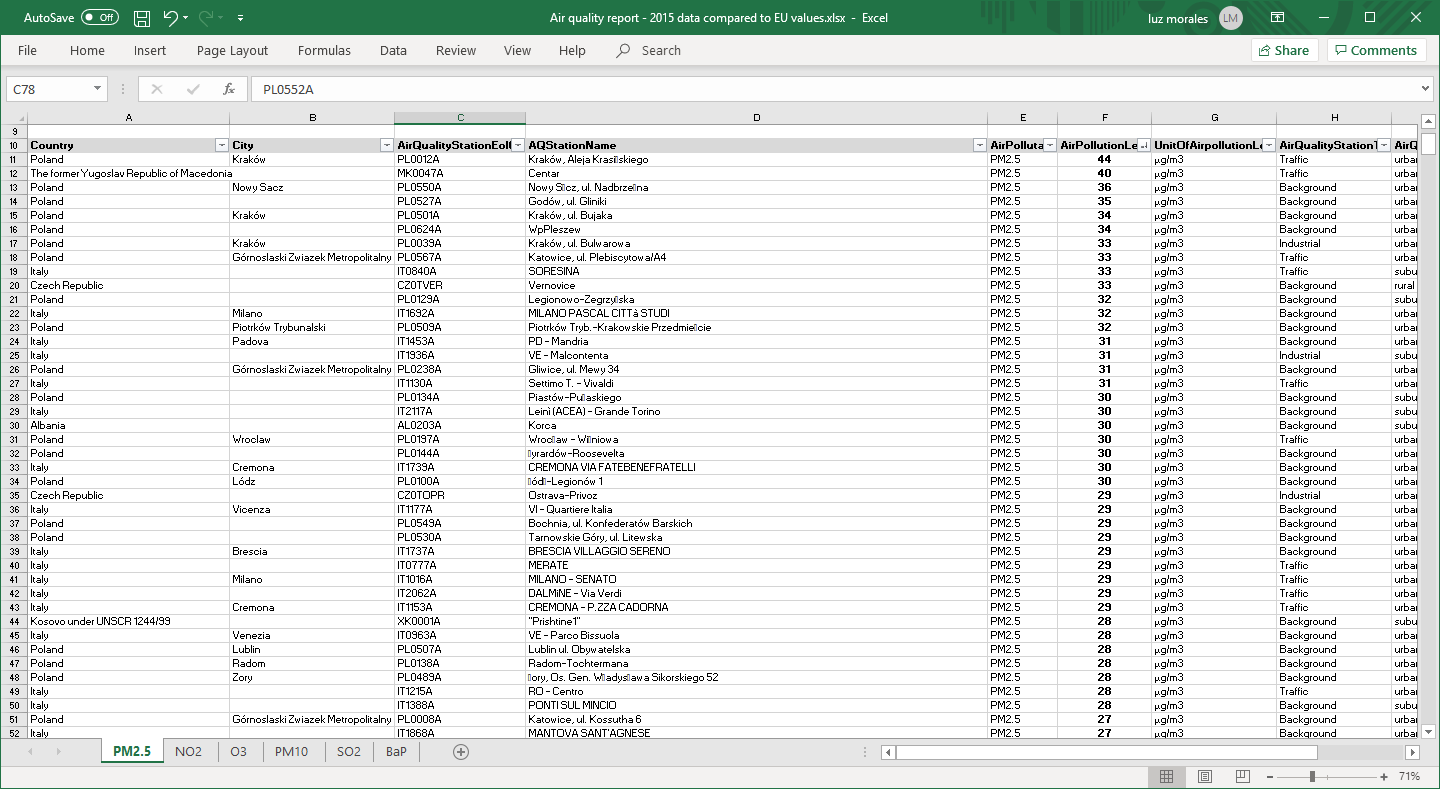
\includegraphics[width=7cm]{ExampleOpenDataEuropean}}
    \caption{Open Data Examples}
\end{figure}

    

    
\subsubsection{How to solve it} 
Through a series of processes such as extraction, transformation and
cleaning of the data, we obtain the data that is needed according to our design. These processes can arrive
to be very tedious if you do not automate.

\subsubsection{How we solve it. Aire Guru} 

The extracted data is in GeoJSON format, this format provides a JSON object with nested subdocuments, each of these
subdocuments contains a set of data in key form value.
In the following figure we can see the beginning of the document downloaded on June 9, 2019
\footnote{\url{https://datosabiertos.malaga.eu/recursos/ambiente/calidadaire/calidadaire.json}}\\
\newpage
\begin{figure}[h]
    \centering
   \subfigure[First subdocument]{ \centering 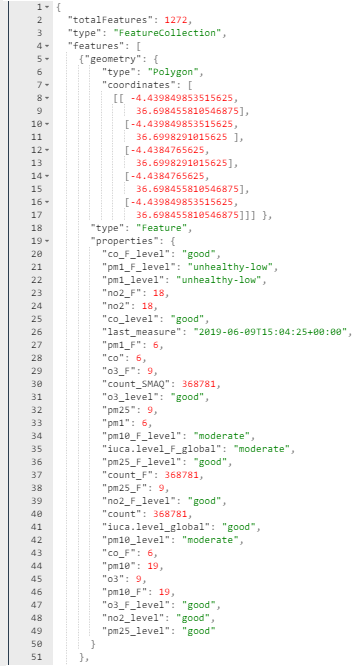
\includegraphics[width=4.75cm]{geoJsonAirQualityData1}}
   \hfill
   \subfigure[Second subdocument]{ \centering 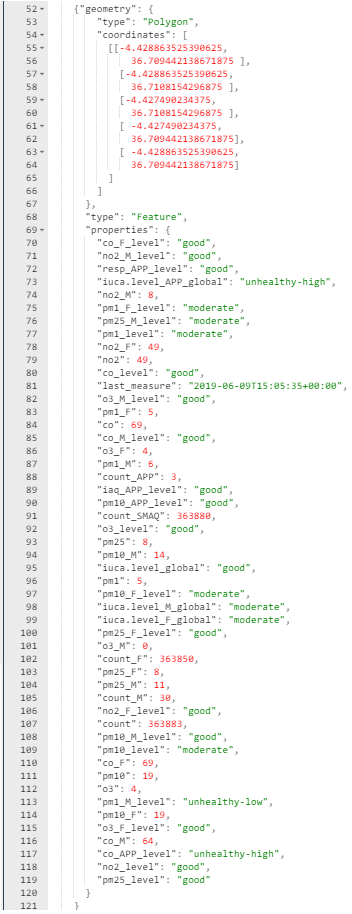
\includegraphics[width=4.75cm]{geoJsonAirQualityData2}}
 
    \caption{Air quality Document [09/06/2019].Open Data Portal Malaga}
    \end{figure}
    
    In this excerpt we can see the first two subdocuments. Each subdocument contains the coordinates of the quality measuring station
    of the air, the date and time when the measurement was recorded and then the values of the measurements.
    In the following figure we can find the description provided by the open data portal.
\begin{figure}[ht]
    \centering
    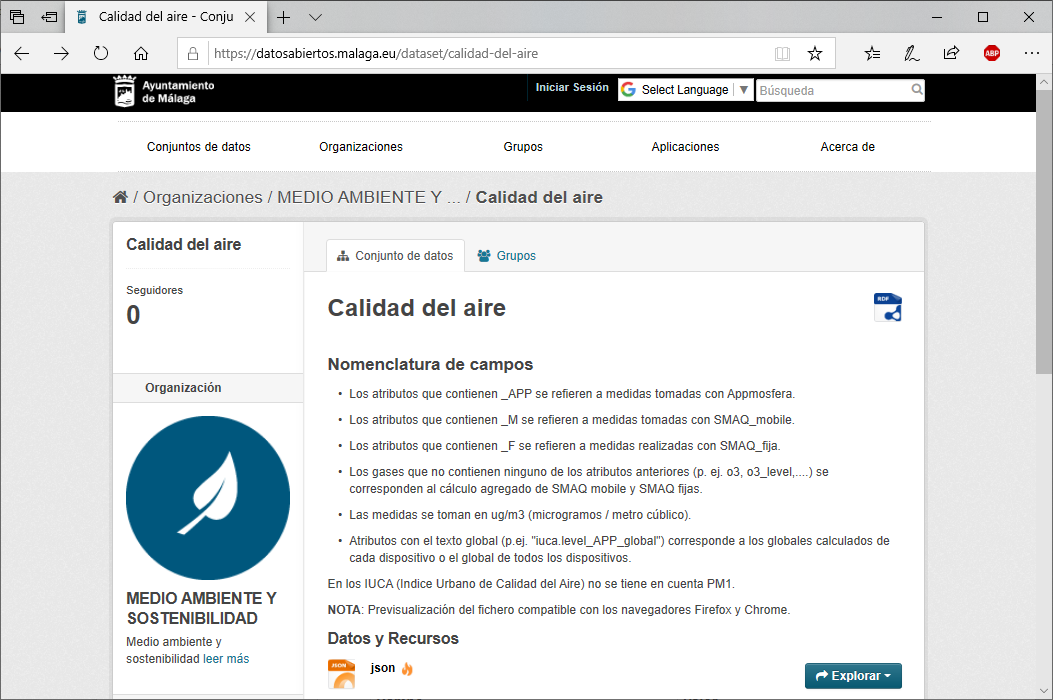
\includegraphics[width=8cm]{geoJsonAirQualityDataDescription}
    \caption{Air quality data description [09/06/2019].Open Data Portal Malaga}
\end{figure}


For a more detailed description of the measures, we have to resort to an external resource, in this case we contacted directly with
the company that installs the UrbanClouds\footnote{\url{https://urbanclouds.city/es/}} measuring stations and provides the data to the Malaga city council.

After selecting the necessary fields according to our design, different cleaning, transformation and extraction tasks have been carried out. \\


\textbf{Cleaning}. Elimination of repeated or non-relevant fields, for example the identifier of the measurement station, since the data set
it contains the coordinates of the station and for us it is much more interesting. \\

\textbf{Transformation}. The values must have an appropriate format to the fields that they represent, for example the date and time in which the measurement has been taken is stored in date format
instead of string as it is provided in the raw data set. \\

\textbf{Extraction}. Selection of the relevant fields. This data set offers one or more measurements for each pollutant, which can be represented by three different fields, a measure
quantitative, a qualitative of the fixed station of measurement and a qualitative station of a mobile station. We will add a field with the measure
more relevant and we will eliminate the others to minimize the processing time. \\

For security, a second totally independent architecture has been implemented that collects the data and stores it raw.

\paragraph{Evaluation} \mbox{} 
\begin{itemize}
    \done We can understand what each one of the fields represented in the data set means thanks to the information
         complementary information presented in the open data portal and by the information provided by the company in charge of
         collect the data.
    \done The data needed for our model has been extracted from the raw data
    
\end{itemize}
\newpage
